\section{Introduction}

It is well known that machine learning (ML) models can yield uncertain and unreliable predictions on out-of-distribution (OOD) inputs, \ie inputs from outside the training distribution~\citep{amodei2016AISafety,goodfellow2015explaining,hendrycks2021many}.
% from an unknown distribution on which the model was not trained~\citep{amodei2016AISafety,goodfellow2015explaining,nguyen2015posterior}.
% The most common practice to avoid such phenomenon is to associate a detector that identifies whether an incoming input is likely to be OOD, then reject the model's decision on the OOD input \citep{hendrycks2018OE,lin2021MOOD,mohseni2020self}.
A common line of defense in this situation is to augment the ML model (\eg a DNN classifier) with a detector that can identify and flag such inputs as OOD~\citep{hendrycks2016msp, liang2018ODIN}. 
The ML model can then abstain from making predictions on such inputs~\citep{tax2008growing, geifman2019selectivenet}.
%~\citep{hendrycks2018OE,lin2021MOOD,mohseni2020self}. 
In many application domains (\eg medical imaging), it is important to understand both the model's prediction as well the reason for abstaining from prediction on certain inputs (\ie the OOD detector's decisions).
Moreover, abstaining from prediction can often have a practical cost, \eg due to service denial or the need for manual intervention~\citep{markoff2016self, mozannar2020consistent}.


Detecting OOD inputs has received significant attention in the literature, and a number of methods exist that achieve strong detection performance on semantic distribution shifts~\cite{yang2021survey, yang2022openood}.
Much of the focus in learning OOD detectors has been on improving their detection performance~\citep{hendrycks2018OE, liu2020energy, mohseni2020self, lin2021MOOD, chen2021atom, sun2021react, cao2022deep}. 
However, the problem of explaining the decisions of an OOD detector and the related problem of designing inherently-interpretable detectors remain largely unexplored (we focus on the former problem). 
A potential approach could be to run an existing explanation method for DNN classifiers with in-distribution (ID) and OOD data separately, and then inspect the difference between the generated explanations. However, it is unclear whether an explanation method that is effective for ID class predictions will also be effective for OOD detection. For instance, feature attributions, the most popular type of explanation \citep{sundararajan2017IG,ribeiro2016LIME}, may not capture visual differences in the generated explanations between ID and OOD inputs~\citep{adebayo2020debugging}.
% , and fail to serve as guidance for humans to determine the trustworthiness of the model ~\citep{adebayo2020debugging}.
Moreover, their explanations based on pixel-level activations may not provide the most intuitive form of explanations for humans.

\begin{figure}[t]
% \vspace{-5mm}
     \centering
     \begin{subfigure}[b]{\columnwidth}
         \centering
         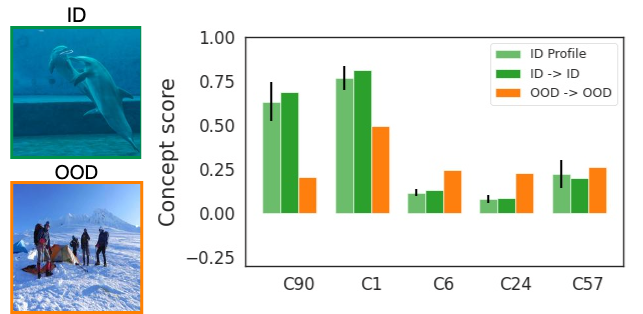
\includegraphics[width=\textwidth]{figures/figure1a.png}
         \caption{\small Correct detection: top dolphin image is correctly detected as ID (dark-green bar), and the bottom image is correctly detected as OOD (orange bar).}
         % ID (or OOD) dolphin image correctly detected as ID (or OOD).
         \label{fig:fig1a}
     \end{subfigure}
     \\
     \vspace{1mm}
     \begin{subfigure}[b]{\columnwidth}
         \centering
         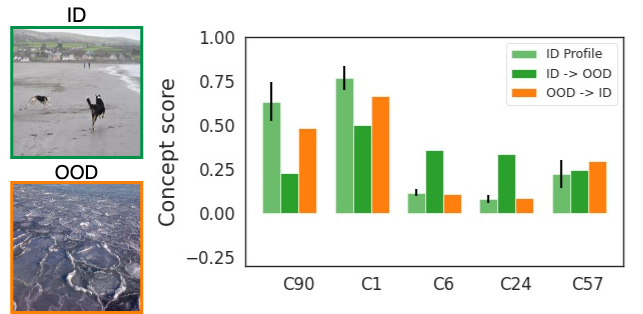
\includegraphics[width=\textwidth]{figures/figure1b.png}
         \caption{\small Wrong detection: top ID image is detected as OOD (dark-green bar), and the bottom OOD image is detected as ID (orange bar).}
         % ID (or OOD) dolphin image falsely detected as OOD (or ID).
         \label{fig:fig1b}
     \end{subfigure}
     \\
     \vspace{1mm}
     \begin{subfigure}[b]{\columnwidth}
         % \centering
         \hspace{1.5mm} 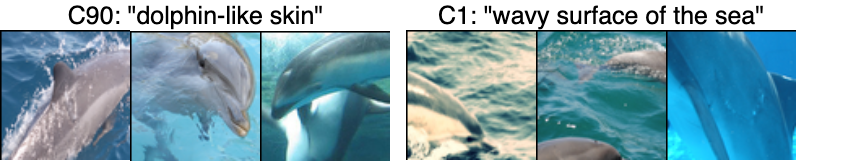
\includegraphics[width=\textwidth]{figures/dolphin_concepts.png}
         \caption{\small Visualization of top-2 important concepts.}
     \end{subfigure}
     \caption{\small \textbf{Our concept-based explanation for the Energy OOD detector~\citep{liu2020energy}.} All input images are classified as ``Dolphin'' but detected differently. On the x-axis of bar graphs, we present the top-5 important concepts that describe the detector's behavior given images classified as ``Dolphin''.
    % Both inputs are classified as "Zebra", but one is detected as ID and the other is detected as OOD by the detector.
    % Even though their class predictions are the same, an OOD-detected input may have very different concept patterns compared to that of an ID-detected input.
    ID profile (light-green) shows the average concept score pattern for ID images predicted as ``Dolphin''. We expect ID inputs predicted into this class to have a similar concept score pattern.}
\vspace{-5mm}
\label{fig:expl-ours-dolphin}
\end{figure}

This paper addresses the above research gap by proposing the first method (to our knowledge) for interpreting the decisions of an OOD detector in a human-understandable way.
We build upon recent advances in concept-based explanations for DNN classifiers~\citep{ghorbani2019ace,zhou2018interpretable,bouchacourt2019educe,yeh2020completeness}, which offer the benefit of providing explanations in terms of high-level {\em concepts} for classification tasks.
% \textcolor{blue}{Our method is unsupervised in that it does not require human-annotations for learning the concepts.}
We focus on extending this explanation framework to the problem of OOD detection.
% We make the first effort at extending their utility to the problem of OOD detection.
As a concrete example, consider Fig.~\ref{fig:expl-ours-dolphin} which illustrates our concept-based explanations given inputs which are all classified as the class ``Dolphin'' by a DNN classifier, but detected as either ID or OOD by an OOD detector.
Our method identifies that the concepts such as C90 ``dolphin-like skin'' and C1 ``wavy surface of the sea'' are key concepts to understand the OOD detector's decisions to tell apart ID and OOD images predicted as ``Dolphin''.
The user can verify that these concepts are aligned with human intuition and the OOD detector relies on them for making decisions.
We also confirm that the OOD detector predicts a certain input as ID when its concept-score patterns are similar to that of normal ID Dolphin images. Likewise, the detector predicts an input as OOD when its concept-score patterns are very different from that of ID inputs from the same class.
% A user can verify whether the OOD detector makes decisions based on the concepts that are aligned with human intuition (\eg ), and that the incorrect detection (as in Figure~\ref{fig:fig1b}) is an understandable mistake, not a misbehavior of the OOD detector.
Our explanations can help a user analyze if an incorrect detection (as in Fig.~\ref{fig:fig1b}) is an understandable mistake or a misbehavior of the OOD detector, evaluate the reliability of the OOD detector, and decide upon its adoption in practice.



% Unfortunately, being a statistical model, any OOD detector can make incorrect decisions, but we argue that it is important for an OOD detector to provide explanations when that occurs. 
% For instance, an OOD detector paired with a medical-diagnosis classifier may consistently detect a specific type of OOD input as ID, although the input may be clearly OOD to a human analyst. In such cases, it would be useful if the human analyst can extract an explanation for the detector's error to provide a better understanding of the detector's behavior.

% \textcolor{blue}{Aside from the }
% \jihye{@jayaram: I added the last sentence to give impression that explanations for OOD detector is helpful not only for misdetection but also for correct detections as well.}

% Recently, there has been an increasing number of works addressing the problem of learning 
% OOD detectors with better performance~\citep{liu2020energy,mohseni2020self,lin2021MOOD}.
% However, the problem of explaining the decisions of an OOD detector remains largely unexplored. Naturally, one may consider running an existing interpretation method for ML models (e.g., \citep{kim2018tcav, ghorbani2019ace}) on an example input, but that is inadequate in that it fails to provide insights as to why one example is ID while another is OOD.


% Extracting concept-based explanations, given any black-box OOD detector, is however challenging.
We aim to design a general interpretability framework that is applicable across a wide range of black-box OOD detectors.
Accordingly, a research question we ask is: {\em without relying on the internal mechanism of an OOD detector, can we identify a good set of concepts that are appropriate for understanding why the OOD detector predicts a certain input to be ID\,/\,OOD?} 
A key contribution of this paper is to show that this can be done unsupervised, without any additional human annotations for interpretation.
%
%with in-distribution and OOD data, respectively, and then inspecting the difference between the two generated explanations.
%Unfortunately, there is no guarantee that a method that can successfully explain a model's predictions can also be effective for OOD detectors.% Such mis-detections can hurt the human's trust in the detection algorithm, thus restricting the future use of the OOD detector in medical diagnosis.
% Having an algorithm that can explain the OOD detector's decisions might reveal that such mis-detected inputs were in-fact very similar to the in-distribution (ID) data.
%
%However, such misdetected OOD inputs could have been genuinely similar to in-distribution data, and those mistakes by the OOD detector would be negligible compared to its benefits. 
%Hence, understanding the behavior of OOD detectors is essential for their widespread adoption to real-world applications.
%
\iffalse

\begin{wrapfigure}{r}{0.5\linewidth}
\begin{center}
% \rule{0.9\linewidth}{0.75\linewidth}
% \begin{figure}[t]
% \vspace{1mm}
% 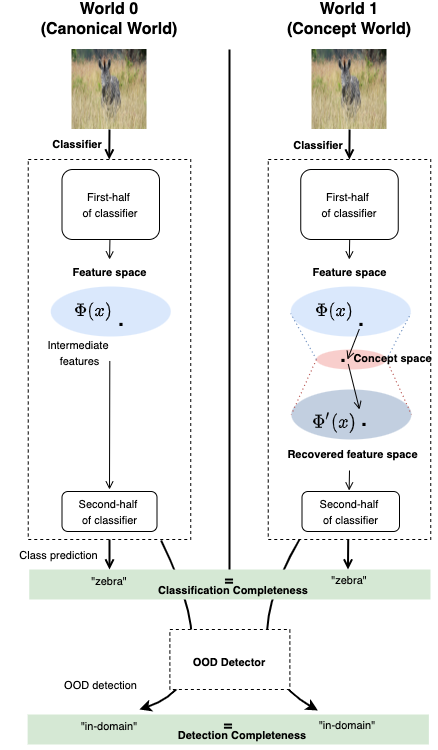
\includegraphics[width=0.45\textwidth]{figures/completeness.png}
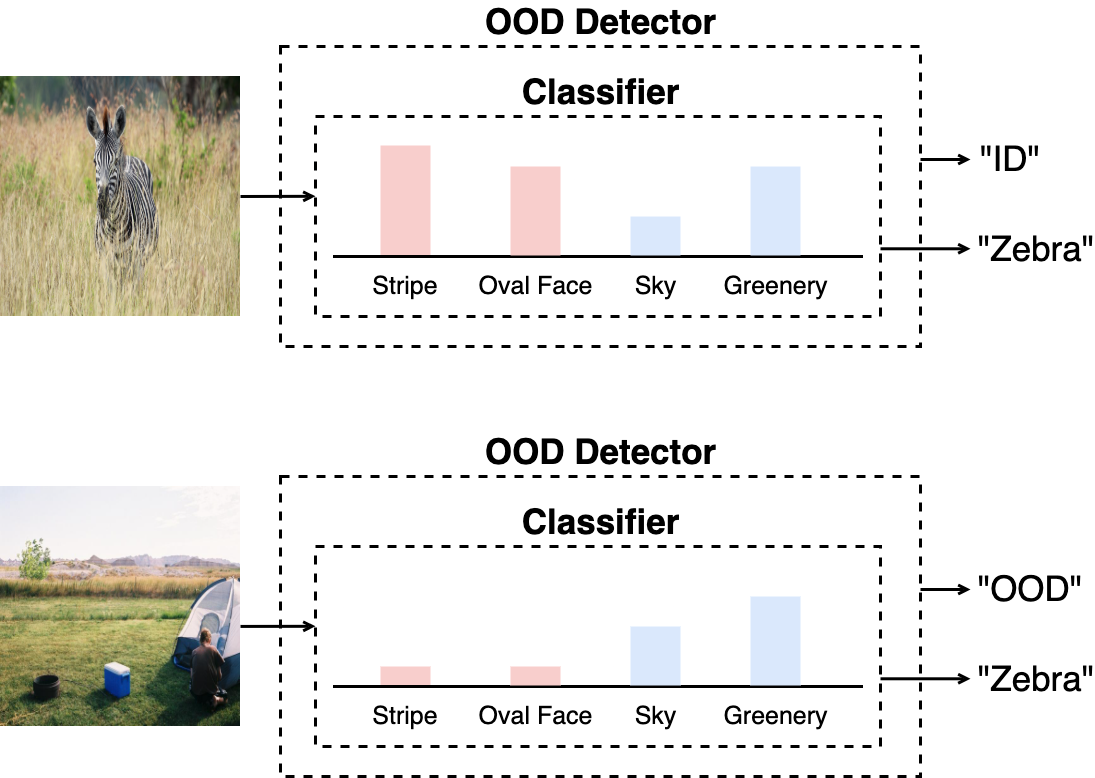
\includegraphics[scale=0.17]{figures/separability.png} 
\vspace{-3mm}
% \vspace{-0.1in}
\caption{\small \textbf{Our concept-based explanation for Energy detector~\citep{liu2020energy}.} "Stripe", "Oval Face", "Sky" and "Greenery" are concepts that completely explain the behavior of the classifier and OOD detector.
% Both inputs are classified as "Zebra", but one is detected as ID and the other is detected as OOD by the detector.
Even though their class predictions are the same, an OOD-detected input may have very different concept patterns compared to that of an ID-detected input.}
% \vspace{-8mm}
\label{fig:detection-separability}
\end{center}
\vspace{-0.12in}
% \end{figure}
\end{wrapfigure}

\begin{figure}[t]
\centering
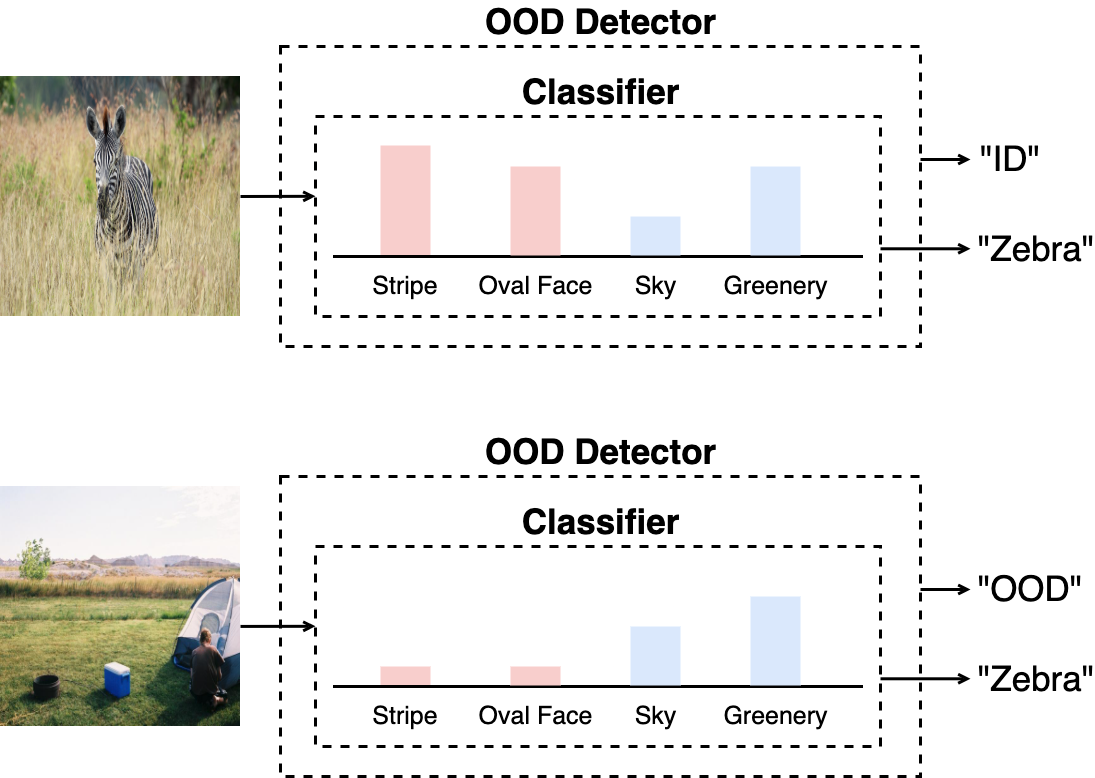
\includegraphics[scale=0.17]{figures/separability.png} 
\caption{ \textbf{Concept-based explanation for OOD detector.} "Stripe", "Oval Face", "Sky" and "Greenery" are concepts that completely explain the behavior of the classifier and OOD detector.
% Both inputs are classified as "Zebra", but one is detected as ID and the other is detected as OOD by the detector.
Even though their class predictions are the same, an OOD-detected input may have very different concept patterns compared to that of an ID-detected input.}
\label{fig:detection-separability}
\end{figure}

\fi
%

In summary, we make the following contributions:
\begin{itemize} [leftmargin=*, topsep=1pt, noitemsep]
% \begin{itemize}
\item We motivate and propose new metrics to quantify the effectiveness of concept-based explanations for a black-box OOD detector, namely \textit{detection completeness} and \textit{concept separability} (Sections \ref{sec:two_worlds}, \ref{sec:completeness_score}, and \ref{sec:separability_score}).  
\item We propose a concept-learning objective with suitable regularization terms that, given an OOD detector for a DNN classifier, learns a set of concepts with high detection completeness and concept separability (Section~\ref{sec:concept_learning});
% \item We introduce regularization terms and propose a method, which given an OOD detector for a DNN classifier, learns a set of concepts that have good detection completeness and concept separability (\S~\ref{sec:concept_learning});
% \item Our empirical results with popular OOD-detectors confirm the insight that concepts with high values for the proposed metrics provide a much clearer distinction for explaining detected-ID and detected-OOD inputs.
\item By treating the OOD detector as a black-box, we show that our approach can be applied to explain a variety of existing OOD detection methods.
% We evaluate the proposed concept learning on popular OOD detectors with multiple real-world datasets. 
We also provide empirical evidence that concepts learned for classifiers cannot be directly used to explain OOD detectors, whereas concepts learned by our method are effective for explaining both the classifier and OOD detector (Section~\ref{sec:eval-concept}).
% which supports the need for our concept discovery method and proposed metrics.
\item By identifying prominent concepts that contribute to an OOD detector's decisions via a modified Shapley value importance score based on the detection completeness, we demonstrate how the discovered concepts can be used to interpret the OOD detector (Section~\ref{sec:expt_concept_based_explanations}).
\end{itemize}


\mypara{Related Work. }  In the literature of OOD detection, recent studies have designed various scoring functions based on the representation from the final or penultimate layers \citep{liang2018ODIN, devries2018learning}, or a combination of different internal layers of a DNN classifier~\citep{lee2018mahalanobis, lin2021MOOD, raghuram2021JTLA}.
A recent survey on generalized OOD detection can be found in Yang et al.~\citep{yang2021survey}. Our work aims to provide post-hoc explanations applicable to a wide range of black-box OOD detectors without modifying their internals.
Among different interpretability approaches, concept-based explanation~\citep{koh2020concept-bottleneck, SENN} has gained popularity as it is designed to be better-aligned with human reasoning \citep{armstrong1983human-concepts,tenenbaum1999concept-learning} and intuition~\citep{ghorbani2019ace,zhou2018interpretable,bouchacourt2019educe,yeh2020completeness}. There have been limited attempts to assess the use of concept-based explanations under data distribution changes such as adversarial manipulation~\citep{kim2018tcav} or spurious correlations~\citep{adebayo2020debugging}.
However, designing concept-based explanations for OOD detection requires further exploration and is the focus of our work.
% Feature attribution is the most commonly used post-hoc explanation method that attributes the decision to local input features~\citep{baehrens2009grad, simonyan2013grad, smilkov2017smoothgrad, sundararajan2017IG}, but recent works have demonstrated its vulnerability to \eg adversarial perturbations~\citep{ghorbani2019fragile,heo2019fooling,slack2020fooling}. 
% \citept{adebayo2020debugging} also conduct experimental analyses and a human subject study to assess the effectiveness of feature attributions under various settings (including on OOD data), and show that feature attributions barely have any visual difference between ID inputs and OOD inputs.
%To the best of our knowledge, we are the first to study concept-based interpretability for explaining the behavior of OOD detectors.
% \textcolor{blue}{Add a pointer to a more detailed related work section in the appendix.}



\iffalse

Once machine learning (ML) model is deployed in real-world settings, it often encounters inadvertent situations.
Specifically, with OOD inputs, drawn from an unknown distribution that the model has not been exposed to during training, it can yield uncertain and unreliable decisions \citep{amodei2016AISafety,goodfellow2015explaining,nguyen2015posterior}.
The most common practice to avoid such phenomenon is to associate a detector that identifies whether an incoming input is likely to be OOD, then reject the model's decision on the OOD input \citep{hendrycks2018OE,lin2021MOOD,mohseni2020self}.
While a plethora of works have focused on bringing better-performing algorithmic approaches for OOD detection, however, there is little effort to reason about their decisions.
Limited understanding of OOD detection results can confine the adoption of the OOD detection methods: for instance, an OOD detector paired with a medical diagnosis model may consistently detect a specific type of OOD data as in-distribution, while those data genuinely share common attributes with in-distribution data.
Even when such misdetection could be reasonably understandable to humans, it could restrict the future use of OOD detection methods in medical diagnosis.
% Hence, it is critical to interpret existing OOD detectors in a human-understandable way.
To this end, we aim to develop an effective method targeted to OOD detector explanations.
% Not limited to simply avoiding misleading behaviors of models, however, to develop better-performing and more reliable models, we need to understand \jihye{reliability of ood detector and its decision.}
% Suppose ...., then a ML practitioner can decide .... to ...(improve) the model \jihye{simple use case of our method}

A natural approach to explain OOD detectors would be running an existing interpretation method with in-distribution and OOD data, respectively, and then inspecting the difference between the two generated explanations \citep{}.
Unfortunately, there is no guarantee that the method that could successfully explain model predictions can also be effective for the use case.
For instance, feature attribution is the most commonly used type of explanation, but it is known to be unreliable even to invisible manipulation of inputs \citep{}
\citep{adebayo2020debugging} study the effectiveness of feature attributions specifically with OOD data through human subject tests and experimental analysis; they show that feature attributions make no visual difference between ID inputs and OOD inputs, and therefore, might not be intuitive guidance for humans when deciding whether to trust model predictions with OOD inputs. 
Other than feature attributions, concept-based explanation is another line of model explanation methods with the advantage of using human-friendly, high-level concepts, but related works have only focused on their usage for understanding model predictions \citep{}.

\jihye{Below are incomplete}

Notwithstanding the rapid growth of ML explainability and the development of high-performance OOD detector, little work has been done to reason about OOD detection.
This paper takes a step toward interpreting what makes data to be detected as in-distribution or OOD, and what are the distinguishing characteristics between in-distribution and OOD data.
% A natural approach would be running an existing explanation method with in-distribution and OOD data, and inspecting the difference between the generated explanations of in-distribution and OOD.
% Unfortunately, one caveat with \jihye{...} is that the method would provide reliable and intuitive explanation with in-distribution inputs, but are not guaranteed to covey reliable, and easy-to-interpret information to reason about the model's behavior given OOD inputs.
% For instance, feature attribution methods \citep{baehrens2009grad, simonyan2013grad, smilkov2017smoothgrad, sundararajan2017IG} that successfully assess relevance of the dimensions of in-distribution input to a model’s output, fail to capture visual distinguishability between in-distribution attribution and OOD attribution \citep{adebayo2020debugging}.
% Moreover, \citep{adebayo2020debugging} shows that explanation by the presentation of visually similar attributions may not be an informative guide for human users to decide the trustworthiness of model decision.
For instance, feature attributions are the most popular local explanation method \citep{baehrens2009grad, simonyan2013grad, smilkov2017smoothgrad, sundararajan2017IG}, but they fail to assist human users' decision on the reliability of model outputs, due to no visual difference between in-distribution and OOD attributions \citep{adebayo2020debugging}. 
Moreover, they are limited to discovering the 

Better aligned with human concept-based thinking \jihye{cite Tenenbaum, Armstrong}, ...
Concept-based explanation characterizes the global behavior of model in terms of intuitive, human-understandable concepts \citep{kim2018tcav, ghorbani2019ace, yeh2020completeness}, but their \textit{appropriateness} for OOD detection tasks are not investigated yet.
We propose to extend their usage to OOD detection, and evaluate the effectiveness/appropriateness? -- in terms of detection completeness and separability.
\jihye{intuition and brief description of detection completeness and separability}.
\jihye{clarification on the meaning of providing explanations for ood detection. It is not our goal to understand the model coverage on ID samples in terms of concepts}
We also extend \citep{yeh2020completeness}'s unsupervised approach to concept discovery to learn a set of concepts with high detection completeness and separability scores.\\
% Motivated by the intuitiveness \jihye{human-understandable? user-friendly?} of concept-based explainability, we aim to extend the use of high-level concepts into OOD detection.
% In this paper, (our goal)
% \jihye{find a set of concepts that are not just completely describing the behavior of DNN classifier, } 
% However, as demonstrated in Section \jihye{()},

WIth the set of concepts, describe what kind of explanations we provide.... \\.\\.\\.\\.\\.\\.\\.

Our contributions can be summarized as follows:
\begin{itemize}[leftmargin=*, topsep=1pt, noitemsep]
    \item Our work is the first quantitative and qualitative evaluation on the appropriateness of high-level concepts toward OOD detection explanation.
    We introduce two metrics for the quantitative evaluation of concepts -- detection completeness and separability.
    \item We propose an unsupervised \jihye{by saying unsupervised, I mean we don't involve extra annotations for concepts} learning framework to find concepts that possess the desired properties.
    \jihye{also, theoretical analysis on how separability in concept scores is related to the separability in OOD scores?}
    \item We verify the effectiveness of our framework to extract concepts for real-world image datasets and popular OOD detectors, and demonstrate insights into the behavior of OOD detectors.
\end{itemize}

\fi